\setcounter{figure}{0}

\section{30th July 2023: Identity in our current times}
\subsection*{Text: No specific text for this week}
  % \begin{quote}
  %   Bible passage goes here
  % \end{quote}
\subsection*{Notes}
\begin{itemize}
  \item{What we take to be our core identity affects what we do in our life. For example, if we take “i am a good husband and a good father” as our core identity, then we would strive to be good husbands and fathers. But if we take “i am a live for the moment, maximise pleasure” as our core identity, then whenever our family doesnt give us joy, we might ditch them.}
  \item{In our life, we have many identities. Who we are at work, our ethnic identity, our political identity, etc. But most of these identities are accidental (i.e, they do not define who we are). Some would say that there is no core identity, but then our identity is just the sum of all these accidental identities. Then when these accidental identities change, our identity changes too. But this sounds quite pessimistic… Furthermore, if these secondary identities conflict, then if there is no core identity, then how? But if there is a core identity, then that would help us determine which conflicting identity to keep or to drop.}
  \item{But as Christians, our view is that there is a core identity, and it is that we are fearfully and wonderfully made by God in God’s image. I.e, our core identity is that we are creatures that are created by a loving God. C.f Genesis 2. You and I are human beings (a unique ensouled body; embodied soul) created in the image of God; known, created, loved and redeemed in the Lord Jesus Christ, even as we take on the many multiple identities that present themselves in our lives.}
  \item{From the christian POV issue, the primary problem is that we \textbf{reject} our God-given core identity, and that we define our own discovered primary personal identity. This is sin! C.f Romans 1. Or, it is that we subordinate our God-given core identity under the secondary identities that might actually come from a good place. For example, there is nothing wrong with liking basketball, but if we take our core identity as “i am a basketball player” more than “i am a creature created lovingly by God to be in fellowship with Him”, then that is sin. And sin here is both dishonouring to God and also destructive to us. When our core identity is gotten rather than given, then we feel the need to maintain our gotten core identity.}
  \item{But the good thing is that God has provided us with a means to \textbf{restore} and \textbf{redeem} the identity that we have all rejected. And that is by giving us His Son.}
  \item{As per Romans 5:12-21, Jesus Christ re-lived Adam's \textit{life}, Jesus Christ died Adam's \textit{death}, and Jesus Christ fulfilled Adam's \textit{destity}.
  \begin{enumerate}
    \item{God in Christ Jesus names and calls us as his own (John 10:14-16)}
    \item{He gives us back our primary identity (created in God's image; known by God; being in Christ)}
    \item{He does this by laying down his life (John 10:17).}
    \item{Such is the worth bestowed on us that comes from the identity God gives to us and Jesus redeems back for us}
  \end{enumerate}
  
  }
  % \item{\begin{figure}[H]
  %   \centering
  %   % 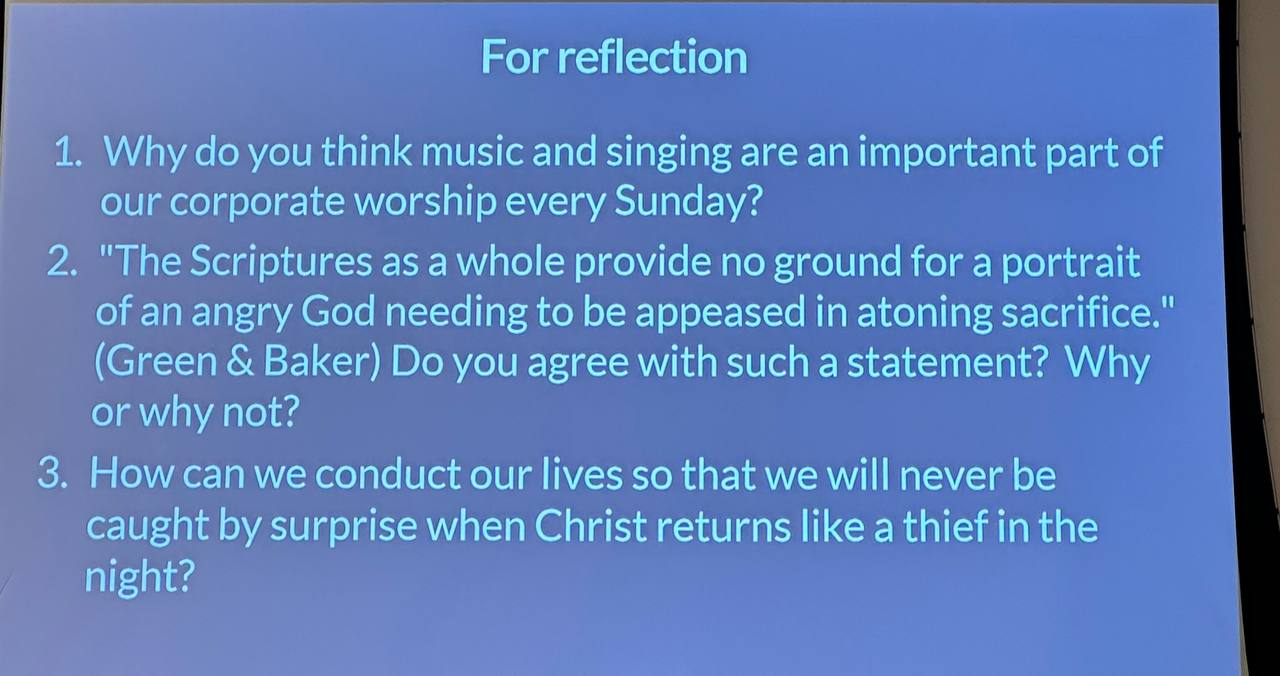
\includegraphics[width=0.8\textwidth, trim={0cm 0cm 0cm 0cm},clip]{Figures/marchSermon4Reflections.jpg}
  %   \includegraphics[width=0.8\textwidth, trim={0cm 0cm 0cm 0cm},clip]{example-image-a}
  %   \caption[]{Reflection questions for this sermon}
  %   \label{}
  % \end{figure}}
\end{itemize}